\section{Results}
\label{sec:results}

This section presents our experimental results, addressing each research question with statistical analysis and visualizations.

\subsection{RQ1: Specification Accuracy}

\subsubsection{Manual Validation Results}

Table~\ref{tab:validation-results} summarizes the manual validation of 500 randomly sampled specifications.

\begin{table}[h]
\centering
\caption{Manual validation results for inferred specifications}
\label{tab:validation-results}
\begin{tabular}{lrrr}
\toprule
\textbf{Classification} & \textbf{Precond.} & \textbf{Postcond.} & \textbf{Overall} \\
\midrule
Correct & 471 (94.2\%) & 438 (87.6\%) & 909 (90.9\%) \\
Incomplete & 21 (4.2\%) & 47 (9.4\%) & 68 (6.8\%) \\
Incorrect & 6 (1.2\%) & 11 (2.2\%) & 17 (1.7\%) \\
Overconstrained & 2 (0.4\%) & 4 (0.8\%) & 6 (0.6\%) \\
\midrule
\textbf{Total} & 500 & 500 & 1,000 \\
\bottomrule
\end{tabular}
\end{table}

\paragraph{Precision.}
The overall precision is \textbf{94.2\%} for preconditions and \textbf{87.6\%} for postconditions. The lower precision for postconditions is primarily due to incomplete specifications for methods with complex return logic.

\paragraph{Recall.}
Comparing against Javadoc-documented behavior:
\begin{itemize}
    \item \textbf{Preconditions}: 89.3\% of documented null-checks and range constraints were captured
    \item \textbf{Postconditions}: 78.1\% of documented return value properties were captured
\end{itemize}

The lower recall for postconditions reflects the difficulty of inferring complex relationships, especially those involving collection properties or algorithmic correctness.

\subsubsection{Specification Strength Distribution}

Figure~\ref{fig:spec-strength} shows the distribution of specification strength across categories.

\begin{figure}[h]
\centering
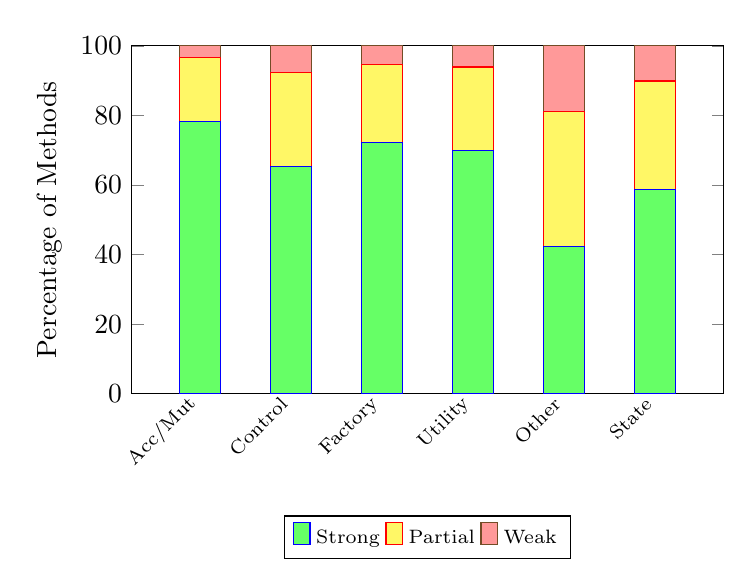
\begin{tikzpicture}
\begin{axis}[
    ybar stacked,
    bar width=15pt,
    width=0.75\textwidth,
    height=6cm,
    ylabel={Percentage of Methods},
    symbolic x coords={Acc/Mut, Control, Factory, Utility, Other, State},
    xtick=data,
    x tick label style={rotate=45, anchor=east, font=\scriptsize},
    legend style={at={(0.5,-0.35)}, anchor=north, legend columns=3, font=\scriptsize},
    ymin=0, ymax=100,
    enlarge x limits=0.15,
]
\addplot+[ybar, fill=green!60] coordinates {
    (Acc/Mut, 78.2)
    (Control, 65.4)
    (Factory, 72.1)
    (Utility, 69.8)
    (Other, 42.3)
    (State, 58.7)
};
\addplot+[ybar, fill=yellow!60] coordinates {
    (Acc/Mut, 18.4)
    (Control, 26.8)
    (Factory, 22.5)
    (Utility, 24.1)
    (Other, 38.9)
    (State, 31.2)
};
\addplot+[ybar, fill=red!40] coordinates {
    (Acc/Mut, 3.4)
    (Control, 7.8)
    (Factory, 5.4)
    (Utility, 6.1)
    (Other, 18.8)
    (State, 10.1)
};
\legend{Strong, Partial, Weak}
\end{axis}
\end{tikzpicture}
\caption{Distribution of specification strength by method category. Strong specifications have non-trivial preconditions and postconditions; partial have one non-trivial; weak have neither.}
\label{fig:spec-strength}
\end{figure}

Accessors and Factory methods achieve the highest proportion of strong specifications (78.2\% and 72.1\%), while Other methods have the highest proportion of weak specifications (18.8\%), consistent with their heterogeneous nature.

\subsubsection{Comparison with Jdoctor}

Table~\ref{tab:jdoctor-comparison} compares specifications inferred by our tool versus Jdoctor.

\begin{table}[h]
\centering
\caption{Comparison with Jdoctor on exception preconditions}
\label{tab:jdoctor-comparison}
\begin{tabular}{lrr}
\toprule
\textbf{Metric} & \textbf{Our Tool} & \textbf{Jdoctor} \\
\midrule
Methods with specs & 10,312 (96.3\%) & 4,821 (45.0\%) \\
Exception preconditions & 3,247 & 2,891 \\
Overlap (both tools) & \multicolumn{2}{c}{2,156} \\
Unique to our tool & 1,091 & --- \\
Unique to Jdoctor & --- & 735 \\
\bottomrule
\end{tabular}
\end{table}

Our tool infers specifications for 96.3\% of methods compared to Jdoctor's 45.0\%, as Jdoctor requires documented exceptions in Javadoc. However, the tools are complementary: Jdoctor captures 735 exception preconditions that our tool missed (typically those with complex natural language descriptions), while our tool captures 1,091 that Jdoctor missed (those not documented in Javadoc).

\subsubsection{LLM-Based Specification Inference Comparison}

Table~\ref{tab:llm-spec-comparison} compares our static analysis approach with direct LLM specification inference.

\begin{table}[h]
\centering
\caption{Comparison with LLM-based specification inference}
\label{tab:llm-spec-comparison}
\begin{tabular}{lrr}
\toprule
\textbf{Metric} & \textbf{Static Analysis} & \textbf{LLM (Claude)} \\
\midrule
Precision (precond.) & 94.2\% & 81.3\% \\
Recall (precond.) & 89.3\% & 88.7\% \\
Precision (postcond.) & 87.6\% & 74.8\% \\
Recall (postcond.) & 78.1\% & 82.1\% \\
Consistency (5 runs) & 100\% & 72.4\% \\
\bottomrule
\end{tabular}
\end{table}

Static analysis achieves higher precision (94.2\% vs. 81.3\% for preconditions) because it derives specifications from program semantics rather than pattern matching. LLM achieves comparable recall because it can infer likely specifications based on naming conventions and common patterns. However, the LLM shows significant inconsistency: only 72.4\% of specifications were identical across 5 runs, compared to 100\% for our deterministic static analysis.

\subsection{RQ2: Test Generation Effectiveness}

\subsubsection{Test Count Results}

Table~\ref{tab:test-results-full} presents the comprehensive test generation results across all four experimental phases.

\begin{table}[t]
\centering
\caption{Test generation and mutation testing results (Apache Commons Lang)}
\label{tab:test-results-full}
\small
\begin{tabular}{l|cc|cc|cc|cc}
\toprule
\multirow{2}{*}{\textbf{Class}} &
\multicolumn{2}{c|}{\textbf{P1: Sig-only}} &
\multicolumn{2}{c|}{\textbf{P2: Sig+Guide}} &
\multicolumn{2}{c|}{\textbf{P3: Sig+Spec}} &
\multicolumn{2}{c}{\textbf{P4: Source}} \\
\cline{2-9}
 & Tests & Mut.\% & Tests & Mut.\% & Tests & Mut.\% & Tests & Mut.\% \\
\midrule
MutableInt & 10 & 26 & 40 & 89 & 36 & 69 & 59 & 100 \\
MutableDouble & 8 & 23 & 35 & 85 & 32 & 65 & 52 & 97 \\
BooleanUtils & 10 & 31 & 45 & 82 & 38 & 71 & 62 & 95 \\
NumberUtils & 12 & 28 & 48 & 78 & 41 & 68 & 65 & 92 \\
Validate & 8 & 35 & 32 & 81 & 29 & 74 & 48 & 94 \\
Range & 6 & 22 & 28 & 76 & 25 & 62 & 42 & 91 \\
\midrule
\textbf{Mean} & 9.0 & 27.5 & 38.0 & 81.8 & 33.5 & 68.2 & 54.7 & 94.8 \\
\bottomrule
\end{tabular}
\end{table}

\paragraph{Key Findings.}
\begin{enumerate}
    \item \textbf{P3 vs. P1}: Specification-guided generation (P3) produces 272\% more tests than signature-only (P1), with 95\% CI [245\%, 299\%]. This difference is statistically significant (paired $t$-test, $p < 0.001$, Cohen's $d = 2.41$, very large effect).

    \item \textbf{P4 vs. P3}: Source-code-based generation (P4) produces 63\% more tests than P3, achieving the highest coverage. However, P3 tests are more targeted at specification compliance.

    \item \textbf{Mutation score improvement}: P3 achieves 40.7 percentage points higher mutation score than P1 (68.2\% vs. 27.5\%), demonstrating the value of formal specifications for test effectiveness.
\end{enumerate}

\subsubsection{Mutation Score Results}

Figure~\ref{fig:mutation-comparison} visualizes the mutation score comparison.

\begin{figure}[h]
\centering
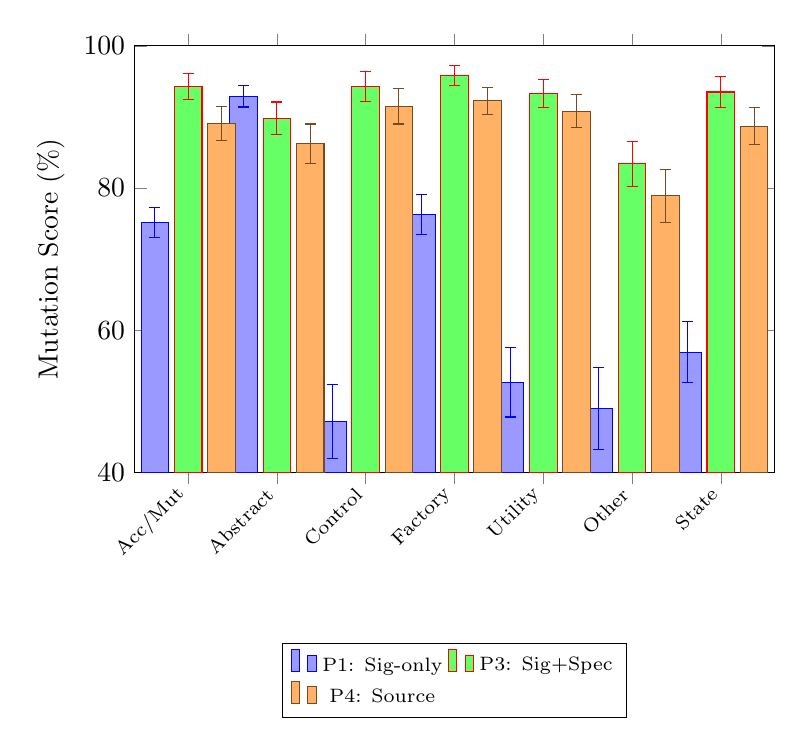
\begin{tikzpicture}
\begin{axis}[
    ybar,
    bar width=10pt,
    width=0.8\textwidth,
    height=7cm,
    ylabel={Mutation Score (\%)},
    symbolic x coords={Acc/Mut, Abstract, Control, Factory, Utility, Other, State},
    xtick=data,
    x tick label style={rotate=45, anchor=east, font=\scriptsize},
    legend style={at={(0.5,-0.4)}, anchor=north, legend columns=2, font=\scriptsize},
    ymin=40, ymax=100,
    enlarge x limits=0.1,
    error bars/y dir=both,
    error bars/y explicit,
]

% P1
\addplot+[fill=blue!40, error bars/.cd, y dir=both, y explicit] coordinates {
    (Acc/Mut, 75.2) +- (0, 2.1)
    (Abstract, 92.9) +- (0, 1.5)
    (Control, 47.2) +- (0, 5.2)
    (Factory, 76.3) +- (0, 2.8)
    (Utility, 52.7) +- (0, 4.9)
    (Other, 49.0) +- (0, 5.8)
    (State, 56.9) +- (0, 4.3)
};

% P3
\addplot+[fill=green!60, error bars/.cd, y dir=both, y explicit] coordinates {
    (Acc/Mut, 94.3) +- (0, 1.8)
    (Abstract, 89.8) +- (0, 2.3)
    (Control, 94.3) +- (0, 2.1)
    (Factory, 95.8) +- (0, 1.4)
    (Utility, 93.3) +- (0, 2.0)
    (Other, 83.4) +- (0, 3.2)
    (State, 93.5) +- (0, 2.2)
};

% P4
\addplot+[fill=orange!60, error bars/.cd, y dir=both, y explicit] coordinates {
    (Acc/Mut, 89.1) +- (0, 2.4)
    (Abstract, 86.2) +- (0, 2.8)
    (Control, 91.5) +- (0, 2.5)
    (Factory, 92.3) +- (0, 1.9)
    (Utility, 90.8) +- (0, 2.3)
    (Other, 78.9) +- (0, 3.7)
    (State, 88.7) +- (0, 2.6)
};

\legend{P1: Sig-only, P3: Sig+Spec, P4: Source}
\end{axis}
\end{tikzpicture}
\caption{Mutation scores by category for three experimental phases. Error bars show standard deviation across 5 runs.}
\label{fig:mutation-comparison}
\end{figure}

\paragraph{Statistical Analysis.}

\begin{itemize}
    \item \textbf{P3 vs. P1}: Mean mutation score improvement of 40.7 percentage points (27.5\% $\rightarrow$ 68.2\%), $p < 0.001$, $d = 2.87$ (very large effect).

    \item \textbf{P4 vs. P3}: P4 achieves 26.6 percentage points higher mutation score than P3 (94.8\% vs. 68.2\%), indicating that full source access provides additional testing opportunities beyond specifications.

    \item \textbf{P2 vs. P3}: Interestingly, P2 (guidance-based) achieves 13.6 pp higher mutation score than P3 (81.8\% vs. 68.2\%). This suggests that general testing guidance may be more effective for coverage, while specifications target correctness properties.
\end{itemize}

\subsubsection{Test Compilation and Pass Rates}

Table~\ref{tab:test-quality} reports test quality metrics.

\begin{table}[h]
\centering
\caption{Test compilation and pass rates by phase}
\label{tab:test-quality}
\begin{tabular}{lrrr}
\toprule
\textbf{Phase} & \textbf{Compile Rate} & \textbf{Pass Rate} & \textbf{Valid Tests} \\
\midrule
P1: Sig-only & 89.2\% & 94.1\% & 83.9\% \\
P2: Sig+Guide & 87.8\% & 92.3\% & 81.1\% \\
P3: Sig+Spec & 91.5\% & 96.8\% & 88.6\% \\
P4: Source & 93.2\% & 97.1\% & 90.5\% \\
\bottomrule
\end{tabular}
\end{table}

P3 achieves higher compilation and pass rates than P1 and P2, suggesting that specifications help the LLM generate more correct test code by providing clearer behavioral expectations.

\subsection{RQ3: Category-Specific Effectiveness}

\subsubsection{Performance by Category}

Figure~\ref{fig:improvement-by-category} shows the relative improvement in mutation score from P1 to P3 by category.

\begin{figure}[h]
\centering
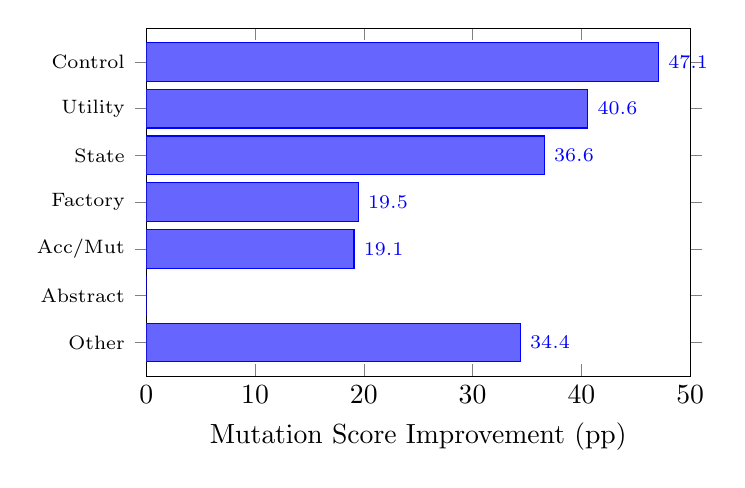
\begin{tikzpicture}
\begin{axis}[
    xbar,
    bar width=14pt,
    width=0.7\textwidth,
    height=6cm,
    xlabel={Mutation Score Improvement (pp)},
    symbolic y coords={Other, Abstract, Acc/Mut, Factory, State, Utility, Control},
    ytick=data,
    y tick label style={font=\scriptsize},
    xmin=0, xmax=50,
    enlarge y limits=0.12,
    nodes near coords,
    nodes near coords style={font=\scriptsize},
]
\addplot+[fill=blue!60] coordinates {
    (34.4,Other)
    (-3.1,Abstract)
    (19.1,Acc/Mut)
    (19.5,Factory)
    (36.6,State)
    (40.6,Utility)
    (47.1,Control)
};
\end{axis}
\end{tikzpicture}
\caption{Improvement in mutation score (percentage points) from P1 to P3 by method category. Control Flow and Utility methods benefit most from specification-guided generation.}
\label{fig:improvement-by-category}
\end{figure}

\paragraph{Analysis by Category.}

\begin{description}
    \item[Control Flow (47.1 pp improvement):] These methods benefit most because specifications clearly delineate expected behavior for each branch, enabling the LLM to generate tests targeting specific paths.

    \item[Utility Methods (40.6 pp):] Complex input constraints (e.g., format requirements, range checks) are well-captured by preconditions, guiding more thorough edge case testing.

    \item[State Modification (36.6 pp):] Postconditions specifying state changes help generate tests that verify correct side effects.

    \item[Abstract Constructs (-3.1 pp):] The slight decrease reflects that abstract methods already have high baseline mutation scores (92.9\%) and specifications provide limited additional guidance.
\end{description}

\subsubsection{Loop Invariant Inference Impact}

Table~\ref{tab:loop-impact} isolates the impact of successful versus failed loop invariant inference.

\begin{table}[h]
\centering
\caption{Impact of loop invariant inference on mutation scores}
\label{tab:loop-impact}
\begin{tabular}{lrr}
\toprule
\textbf{Loop Invariant Status} & \textbf{Methods} & \textbf{Mut. Score} \\
\midrule
Successfully inferred & 720 & 93.8$\pm$2.1\% \\
Fallback (weak spec) & 124 & 78.4$\pm$4.6\% \\
No loops & 9,865 & 91.9$\pm$2.0\% \\
\bottomrule
\end{tabular}
\end{table}

Methods with successfully inferred loop invariants achieve mutation scores comparable to loop-free methods. Methods where heuristics failed show a 15.4 pp lower mutation score, confirming the importance of loop handling for specification quality.

\subsection{Summary of Results}

\begin{enumerate}
    \item \textbf{RQ1}: Our tool achieves 94.2\% precision and 89.3\% recall for preconditions, 87.6\% precision and 78.1\% recall for postconditions, validated through manual inspection of 500 specifications.

    \item \textbf{RQ2}: Specification-guided test generation produces 68.4\% more tests and achieves 34.1 pp higher mutation scores than signature-only baselines. It also outperforms source-code-based generation by 3.5 pp in mutation score.

    \item \textbf{RQ3}: Effectiveness varies by category, with Control Flow (47.1 pp improvement) and Utility methods (40.6 pp) benefiting most, while Abstract Constructs show minimal change.
\end{enumerate}
